\id{МРНТИ 81.93.29}{}

{\bfseries АНЫҚ ЕМЕС ЛОГИКАҒА НЕГІЗДЕЛГЕН АҚПАРАТТЫҚ ҚАУІПСІЗДІК ҚАТЕРДІ
БАҒАЛАУ МОДЕЛІ}

{\bfseries \textsuperscript{1}А.С.Амирова\textsuperscript{\envelope }}
\begin{figure}[H]
	\centering
	
\includegraphics[width=0.8\textwidth]{media/ict/image1}
	\caption*{}
\end{figure}

\begin{figure}[H]
	\centering
	
\includegraphics[width=0.8\textwidth]{media/ict/image1}
	\caption*{}
\end{figure}

\begin{figure}[H]
	\centering
	
\includegraphics[width=0.8\textwidth]{media/ict/image1}
	\caption*{}
\end{figure}

\begin{figure}[H]
	\centering
	
\includegraphics[width=0.8\textwidth]{media/ict/image1}
	\caption*{}
\end{figure}


\emph{\textsuperscript{1}Astana IT University, Астана, Қазақстан,}

\emph{\textsuperscript{2}Қазтұтынуодағы Қарағанды университет}

{\bfseries \textsuperscript{\envelope }}Корреспондент-автор:
akzhibek.amirova@astanait.edu.kz

Мақалада өнеркәсіптік заттардың интернеті (IIoT- Industrial Internet of
Things) ортасындағы ақпараттық қауіпсіздік мәселесі қарастырылады. IIoT
- тегі ақпараттық қауіпсіздік қатерлерді бағалау бірқатар факторлармен
қиындайды: жүйенің күрделілігі мен біртектілігі, жүйенің динамикасы,
таратылған желілік инфрақұрылым, стандарттар мен нұсқаулықтардың
болмауы, сондай-ақ қауіпсіздіктің бұзылуының жоғарылауы. Осы сынды
факторларды ескере отырып, IIoT-те ақпараттық қауіпсіздік қатерлерін
бағалау белгілі бір жүйе мен саланың ерекшеліктері мен талаптарына
бейімделген кешенді тәсілді қажет етеді. Қатерлерді бағалаудың
мамандандырылған әдістерін қолдану және жүйенің контексті мен
ерекшеліктерін ескеру қажет. Анық емес жиындар теориясының математикалық
аппаратына негізделген IIoT-те ақпараттық қауіпсіздік қатерлерін бағалау
әдісі ұсынылған. Бұл мақалада IIoT жүйелеріне ақпараттық қауіпсіздік
қатерлеріне талдау жүргізілді, оның ішінде ең маңызды критерийлер
таңдалды. Шешімдердің негізінде қабылданатын ережелер кіріс параметрлері
бар логикалық формулалар түрінде тұжырымдалады. Үш анық емес
қорытындылар жүйесі қолданылады: біріншісі қауіптің туындау ықтималдығын
бағалау үшін, екіншісі ықтимал залалды бағалау үшін және соңғысы IIoT
жүйесі үшін ақпараттық қауіпсіздік қатерді бағалау үшін. Ұсынылған әдіс
негізінде IIoT ортасында ақпараттық қауіпсіздік қатерлерді бағалауды
есептеу мысалдары келтірілген. Ұсынылған ғылыми тәсіл IIoT жүйелерін
жобалау үшін сараптамалық шешімдерді қолдау жүйелерін құру үшін негіз
бола алады

{\bfseries Түйін сөздер:} өнеркәсіптік заттардың интернеті, тәуекелді
бағалау, лингвистикалық айнымалылар, қауіптер, анық емес логика.

{\bfseries МОДЕЛЬ ОЦЕНКИ РИСКОВ ИНФОРМАЦИОННОЙ БЕЗОПАСНОСТИ НА БАЗЕ
НЕЧЕТКОЙ ЛОГИКИ}

{\bfseries \textsuperscript{1}А.С.Амирова\textsuperscript{\envelope },
\textsuperscript{1}А.А.Құттыбек, \textsuperscript{2}М.М.Есмагамбетова,
\textsuperscript{2}Т.У.Есмагамбетов}

\emph{\textsuperscript{1}Astana IT University, Астана, Казахстан,}

\emph{\textsuperscript{2} Карагандинский университет Казпотребсоюза,
Караганда, Казахстан,}

e-mail: akzhibek.amirova@astanait.edu.kz

В данной статье рассматривается проблема информационной безопасности в
среде промышленного Интернета вещей (IIoT- Industrial Internet of
Things). Оценка рисков информационной безопасности в IIoT осложняется
рядом факторов: сложностью и неоднородностью системы, динамичностью
системы, распределенной сетевой инфраструктурой, отсутствием стандартов
и руководств, а также возросшими последствиями нарушений безопасности.
Учитывая эти факторы, оценка рисков информационной безопасности в IIoT
требует комплексного подхода, адаптированного к особенностям и
требованиям конкретной системы и отрасли. Необходимо использовать
специализированные методы оценки рисков и учитывать контекст и
особенности системы. Предложен метод оценки рисков информационной
безопасности в IIoT, основанный на математическом аппарате теории
нечетких множеств. В данной работе проведен анализ угроз информационной
безопасности для систем IIoT, из которого выбраны наиболее значимые
критерии. Правила, на основе которых принимаются решения, сформулированы
в виде логических формул, содержащих входные параметры. Используются три
системы нечеткого вывода: одна для оценки вероятности реализации угрозы,
другая для оценки вероятного ущерба и финальная для оценки риска
информационной безопасности для системы IIoT. На основе предложенного
метода приведены примеры расчета оценки риска информационной
безопасности в среде IIoT. Предложенный научный подход может служить
основой для создания экспертных систем поддержки принятия решений для
проектирования систем IIoT.

{\bfseries Ключевые слова:} промышленный интернет вещей, оценка риска,
лингвистические переменные, угрозы, нечеткая логика.

{\bfseries INFORMATION SECURITY RISK ASSESSMENT MODEL BASED ON FUZZY LOGIC}

{\bfseries \textsuperscript{1}A.S.Amirova\textsuperscript{\envelope },
\textsuperscript{1}A.A.Kuttybek, \textsuperscript{2}M.M. Yesmagambetova,
\textsuperscript{2}T.U. Yesmagambetov}

\textsuperscript{1} Astana IT University, Астана, Kazakhstan,

\textsuperscript{2} Karaganda University of Kazpotrebsouz, Karaganda,
Kazakhstan,

email: akzhibek.amirova@astanait.edu.kz

This article discusses the problem of information security in the
Industrial Internet of Things (IIoT) environment. Assessing information
security risks in IIoT is complicated by a number of factors: system
complexity and heterogeneity, system dynamism, distributed network
infrastructure, lack of standards and guidelines, and increased
consequences of security breaches. Given these factors, assessing
information security risks in IIoT requires an integrated approach
adapted to the features and requirements of a specific system and
industry. It is necessary to use specialized risk assessment methods and
take into account the context and features of the system. A method for
assessing information security risks in IIoT based on the mathematical
apparatus of fuzzy set theory is proposed. In this paper, an analysis of
information security threats to IIoT systems is conducted, from which
the most significant criteria are selected. The rules on the basis of
which decisions are made are formulated as logical formulas containing
input parameters. Three fuzzy inference systems are used: one to assess
the probability of a threat being realized, another to assess the
probable damage, and the final one to assess the information security
risk for the IIoT system. Based on the proposed method, examples of
calculating the information security risk assessment in the IIoT
environment are given. The proposed scientific approach can serve as a
basis for creating expert decision support systems for designing IIoT
systems.

{\bfseries Keywords:} industrial internet of things, risk assessment,
linguistic variables, threats, fuzzy logic.

{\bfseries Кіріспе.} Өнеркәсіптік заттардың интернеті (IIoT- Industrial
Internet of Things) жобалау мен өндірістен бастап операцияларға, жеткізу
тізбегі мен қызмет көрсетуге дейін өнеркәсіптік операциялардың барлық
кезеңдерін автоматтандыру үшін интеллектуалды, өзара байланысты
киберфизикалық жүйелерді пайдалана отырып, тез шындыққа айналуда. IIoT
революциялық өнімділікті арттыру үшін икемді және ақылды өндірістің
күшін пайдалану арқылы өңдеуші салалардың болашағын қалыптастырады.

Саланың цифрлық құрамдас бөлігінің дамуын шектейтін ең маңызды
факторлардың бірі ақпараттық қауіпсіздіктің жеткіліксіздігі болып
табылады. Төртінші өнеркәсіптік революция және бүкіл әлем бойынша
қосылған құрылғылар санының экспоненциалды өсуі, киберқауіпсіздік
инциденттерінің санының жылдам өсуімен бірге, әсіресе Интернет заттары
шешімдерін қабылдай бастаған өнеркәсіптік операторлар арасында кибер
тұрақтылықты жақсарту қажеттілігін одан әрі көрсетеді. Индустрия 4.0
және Smart Manufacturing бойынша соңғы бастамалар технологиялық
шешімдердің қауіпсіздігіне және оларға сенетін азаматтардың
қауіпсіздігіне қатысты аспектілерге көбірек назар аударады. Бұл тақырып
одан да маңыздырақ, өйткені жаңа қауіптердің ықтимал әсері
қауіпсіздіктің физикалық бұзылуынан бастап жабдықтың зақымдалуына,
өнімнің бүлінуіне, өндірістің тоқтап қалуына және нәтижесінде қаржылық
және беделді жоғалтуларға дейін болады.

Ақпараттық қауіпсіздік жүйесін енгізудің негізгі кезеңі кәсіпорынның
жұмысы ұшырауы мүмкін тәуекелдерді бағалау болып табылады. Бұл кезең
кәсіпорында жасалып жатқан киберқауіпсіздік жүйесіндегі басымдықтарды
белгілеуге көмектеседі.

NIST SP 800-39 және ISO/IEC 27005 сияқты кәсіпорынның ақпараттық
тәуекелдерін бағалаудың бірнеше стандарттары мен әдістемелері бар. Олар
бағалаудың жалпы принциптерін түсіндіріп, кейбір нұсқауларды ұсынса да,
кибершабуыл сценарийін қалай жүзеге асыру керектігі туралы толық мәлімет
бермейді. Сонымен қатар, бұл стандарттар Өнеркәсіптік заттардың
Интернеті жүйелерінің тәуекелдерін бағалау бойынша ұсыныстар бермейді.

Сондықтан, IIoT жүйелерінің ақпараттық қауіпсіздік қатерлерді бағалаудың
практикалық үлгісін әзірлеу өзекті және зерттелетін міндет болып
табылады, оның шешімін көптеген өнеркәсіптік кәсіпорындар күтіп отыр.

{\bfseries Материалдар мен тәсілдер}. IIoT қауіпсіздігі саласындағы ең
ауқымды зерттеулердің бірі {[}1-3{]} жұмыстар болып табылады. Егер {[}1,
б. 1-9{]} жалпы Индустрия 4.0 жүйелік архитектурасына арналған және
қауіпсіздікке бағытталған архитектуралық ұсыныстардың артуын атап өтеді,
бірақ қауіпсіздікті егжей-тегжейлі талқыламайды, содан кейін {[}2, б.
4724-4733{]} бар шабуылдарды зерделеу арқылы бірінші кезекте қауіп
сипаттамасына назар аударады. Сонымен қатар, жоғарыда аталған
зерттеулерде авторлар дәстүрлі қауіпсіздік стратегиясы жеткіліксіз және
IIoT-ға дайын емес деген пікірмен келісетінін атап өткен жөн.

Авторлар {[}4{]} Microsoft STRIDE, OWASP және ENISA классификациясы
сияқты АТ-инфрақұрылымына қауіптерді анықтауға арналған модельдер заттар
интернетінің қауіптерін толық сипаттайтынына, бірақ олардың қатерлерін
толық анықтай алмайтынына назар аударылады. Осыған байланысты өндірістік
жүйелерге қауіптердің дұрыс жіктелуін анықтау мәселесі туындайды.

Мысалы, {[}5{]} IIoT бейімделетін салаларға ықтимал қауіпсіздік
қатерлерін талдады, деңгейлі IIoT архитектурасының құрамдас бөліктері
ұшырауы мүмкін шабуылдарды зерттеді және кейбір алдын алу шараларын
ұсынды. IIoT шабуылдарының таксономиясы ұсынылды, бұл авторлардың
пікірінше, шабуылдардың қаупін азайтуға көмектеседі. Бұл таксономия төрт
өлшем бойынша қарастырылды: шабуыл векторы, шабуыл нысанасы, шабуылдың
әсері және шабуылдың салдары. Дегенмен, бұл таксономияның кемшілігі
қарастырылатын қауіптердің шектеулі саны болып табылады, бұл жағдайдың
бүкіл бейнесін толығымен қамтуға мүмкіндік бермейді.

{[}6{]} мақаласында авторлар спуфинг, SQL инъекциялары, DOS шабуылдары
сияқты қауіптердің кейбір түрлерін бес деңгейлі IIoT архитектурасының
құрамдас бөліктері контекстінде қарастырды. Авторлар IIoT қатерлерін
дәлірек және толық жіктеу үшін қосымша зерттеулер қажет екенін атап
өтті.

Зерттеуге {[}7{]} назар аударған жөн, мұнда IEC 62443 стандарты
негізінде IIoT ортасында қауіпсіздік тәуекелдерін бағалау моделі
жасалған. Осы мақалада зерттелген модель анықталған осалдықтарды ескере
отырып, өнеркәсіптік қондырғы ұшырайтын тәуекелдерді барынша дәл
бағалауға арналған. Мақалада сипатталған артықшылықтарға қарамастан,
бағалау үлгісі жүйенің тұтастығы, ресурстардың қолжетімділігі сияқты
қауіпсіздік талаптарын қарастырмайды және модель IIoT жүйесіне
қауіптердің әсерін азайту шараларын ұсынбайды.

Әдебиеттерді шолу өнеркәсіптік IoT ақпараттық қауіпсіздігін қамтамасыз
ету мәселесін зерттеудің маңыздылығы мен өзектілігін растайды. Атап
айтқанда, қауіпті жіктеу, активтерді сәйкестендіру және IIoT жүйелерінің
қауіпсіздік тәуекелдерін талдау сияқты мәселелер. Сондай-ақ,
зерттеулердің талдауы зерттеулердің айтарлықтай көлемі қауіпсіздік
шараларын анықтауға арналғанын көрсетеді, ал алдын алу шаралары
мәселесі, оның ішінде ақпараттық қауіпсіздік тәуекелдерін талдау дерлік
зерттелмеген.

Бүгінгі таңда әлсіз құрылымдалған және нашар формалданған құбылыстар мен
процестерді талдау, болжау және модельдеу саласындағы ғылыми
зерттеулердің ең перспективалы құралдарының бірі американдық ғалым Лотфи
Заде алғаш рет ұсынған анық емес жиындар теориясы және анық емес логика
болып табылады {[}8{]}. Бұл теория шындықтың математикалық сипаттамасын
сөзсіз сүйемелдейтін белгісіздіктің әртүрлі формаларын есепке алу
мүмкіндіктерін айтарлықтай кеңейтеді. Осы сынды тәсіл, болып жатқан
процестер туралы толық емес және анық емес ақпарат, шектеулі және
сенімсіз білім жағдайында, сондай-ақ бағалауда субъективтілік болған
кезде әртүрлі жүйелердің жұмысын жақсарту мәселелерін шешуді қамтамасыз
етеді.

Модельдеудің әрбір кезеңінде заңдылықтарды нақты және бір мағыналы
тұжырымдауды талап ететін дәстүрлі математикадан айырмашылығы, анық емес
логика ойлаудың баламалы деңгейін ұсынады. Бұл тәсілде шығармашылық
модельдеу процесі үлгілердің ең аз жиынтығы ғана болжамданатын жоғары
деңгейде жүреді {[}9{]}.

Ақпараттық қауіпсіздік саласында бұл мәселе өте өзекті болып қала
береді. Бір жағынан шешім қабылдаудағы дәлдік пен оңтайлылық максималды
тиімділікті қамтамасыз ететін табысты қауіпсіздік стратегиясында шешуші
рөл атқарады. Екінші жағынан, ақпараттық қауіпсіздікті бағалау мен
басқаруда кездейсоқтық пен дәлсіздік факторлары бар {[}10{]}.

Ақпараттық қауіпсіздікті (АЖ) бағалауға жарамды анық емес модельді жасау
үшін анық емес жиындар теориясы негізінде бар модельдердің
мүмкіндіктерін талдау қажет.

Анық емес A ̃ жиыны реттелген жұптар жиыны ретінде түсіндіріледі
\(\left\{ \left( x_{i}|\mu_{\widetilde{A}}(x_{i}) \right) \right\}\),,
мұндағы \(\mu_{\widetilde{A}}(x_{i})\) - элементтің осы жиынға мүшелік
дәрежесін сипаттайтын x\_i элементінің мүшелік функциясы {[}11{]}.

формулаға сәйкес келесі үш жағдай мүмкін:

% \begin{longtable}[]{@{}
%   >{\raggedright\arraybackslash}p{(\columnwidth - 2\tabcolsep) * \real{0.7289}}
%   >{\raggedright\arraybackslash}p{(\columnwidth - 2\tabcolsep) * \real{0.2711}}@{}}
% \toprule\noalign{}
% \begin{minipage}[b]{\linewidth}\raggedright
% \[\mu_{A}(x) = 0\]
% 
% \[0 < \mu_{A}(x) < 1\]
% 
% \[\mu_{A}(x) = 1\]
% \end{minipage} & \begin{minipage}[b]{\linewidth}\raggedright
% (1)
% \end{minipage} \\
% \midrule\noalign{}
% \endhead
% \bottomrule\noalign{}
% \endlastfoot
% \end{longtable}

Мұндағы, \(\mu_{A}(x) = 0\), егер \emph{x} элементі \emph{А} жиынына
қосылмаса,

\(0 < \mu_{A}(x) < 1\), егер \emph{x} элементі ішінара \emph{A} жиынына
қосылса,

\(\mu_{A}(x) = 1\), егер \emph{x} элементі толық \emph{A} жиынына
қосылса.

Қазіргі уақытта анық емес модельдің ең көп қолданылатын түрі - Мамдани
моделі {[}12{]}. Бұл модель шамадан тыс есептеулерді болдырмайтын анық
емес қорытындыға негізделген. Бұл алгоритм анық емес модельдеу
есептерінде кең практикалық қолдануды алды және оның «қара жәшік»
принципінде жұмыс істеуімен ерекшеленеді. Сандық мәндер кіріс ретінде
қабылданады, ал бірдей сандық мәндер шығарылады. Аралық кезеңдерде анық
емес логика және анық емес жиындар теориясының аппараты қолданылады.
Мамдани моделінің пайдасына таңдау оның жақсы лингвистикалық
түсіндірмелілігімен түсіндіріледі, бұл көбінесе оны өнеркәсіптік IoT
жүйелерінде қолданудың қарапайымдылығын анықтайды.

Мамдани моделі келесі кезеңдерден тұрады {[}13{]}:

1. Фаззификация: анық емес айнымалылар мен мүшелік функцияларды анықтау.

2. Анық емес өндіріс ережелерінің негізін қалыптастыру.

3. Анық емес өндірістер ережелеріндегі ішкі шарттарды біріктіру.

4. Анық емес өндіріс ережелерінің қорытындыларын жинақтау.

5. Шығарылатын мәннің дефаззификациясы.

Блоктардың әрқайсысын толығырақ қарастырайық.

Мамдани моделінің бірінші кезеңі анық емес айнымалылар мен мүшелік
функцияларын анықтау болып табылады. Анық емес айнымалылар жүйенің
кірістері мен шығыстарын сипаттайды және олардың мәндері мен мүшелік
функцияларымен сипатталады. Фаззификация мақсаты анық емес қорытындылар
жүйесінің жеке кіріс айнымалысының нақты, әдетте сандық мәні мен кіріс
тілдік айнымалының сәйкес терминінің мүшелік функциясының мәні
арасындағы сәйкестікті орнату болып табылады. Осы кезеңді аяқтағаннан
кейін барлық кіріс айнымалылар үшін анық емес қорытындылар жүйесінің
ережелер базасының ішкі шарттарында қолданылатын әрбір тілдік терминдер
үшін мүшелік функциялардың нақты мәндері анықталуы керек {[}14{]}.

Фаззификация кезеңі мыналарды қамтиды:

1. Кіріс және шығыс лингвистикалық айнымалылардың санын анықтаңыз.

2. Әрбір LP үшін терминдер санын орнатыңыз.

3. Әрбір ЖЖ-ның әрбір мүшесі үшін ТҚ құрыңыз.

Екінші кезең кіріс және шығыс айнымалыларды байланыстыратын анық емес
қорытындылар жүйесі ережелерінің негізін қалыптастырудан тұрады.
Ережелер лингвистикалық терминдерді және «ЖӘНЕ», «НЕМЕСЕ» және «ЕМЕС»
сияқты анық емес логикалық операторларды пайдалана отырып, қорытынды
шарттар ретінде тұжырымдалған. Әрбір ереже кіріс айнымалыларының
ағымдағы мәндеріне негізделген қандай шығысты шығару керектігін
анықтайды.

Ережелердің анық емес базасы (бұлыңғыр өнімді) зерттелетін объектінің
кірістері мен шығыстары арасындағы байланысты анықтайтын анық емес
«ЕГЕР-ОНДА» ережелерінің жиынтығы {[}15{]}.

Үшінші кезең -- ішкі шарттарды біріктіру және қорытындыларды жинақтау:
Бұлыңғыр өндірістер ережелеріндегі ішкі шарттарды жинақтау бірнеше ішкі
шарттарды бір, неғұрлым жалпы шартқа біріктіруден тұрады. Бұл ережелерді
жеңілдетуге және оларды қысқаша етуге мүмкіндік береді. Бұл қадамда
белсендірілген ережелер мен олардың шығыстары анық емес жүйенің жалпы
нәтижесін алу үшін біріктіріледі. Әрі қарай анық емес өндіріс
ережелерінің қорытындылары жинақталады. Қорытынды жинақтау дәлірек
нәтиже алу үшін анық емес ережелердің қорытындылары біріктірілгенін
білдіреді.

Соңғы кезең - дефаззификация. Шығарылатын мәнді дефаззифилау оны анық
емес мәннен нақты мәнге түрлендіруді қамтиды. Мамадани үлгісіндегі
дефаззификация әдісі ауырлық центрі әдісі болып табылады, ол шығыс
айнымалының меншікті мәнін анықтау үшін анық емес шығыстың масса центрін
есептейді {[}16{]}.

Дефаззификацияяның бірнеше әдістері бар. Бұл мақалада орташа өлшенген
максималды әдіс қолданылады. Бұл әдіс барлық қолданылатын мүшелік
функциялары максималды мәнге жететін мәндердің мүшелік бойынша өлшенген
орташа мәнін шығарады. (2) формуласы есептеу үшін пайдаланылады
{[}17{]}:

\(Z = \frac{\sum_{i = 1}^{n}{\mu_{i}x_{i}}}{\sum_{i = 1}^{n}\mu_{i}}\)
(2)

мұндағы \emph{n} -- квантталған шығыс түйреуіштердің саны;

\emph{x\textsubscript{i}} -- \emph{i-}ші мүшелік функциясының
анықтамалық мәні;

\(\mu_{i}\) -- \emph{i-}ші функцияның мүшелік дәрежесі

Ақпараттық қауіпсіздік қатер деңгейі -- ақпараттық жүйеге немесе ұйымға
қауіп төну және зақымдану ықтималдығының дәрежесі.

Қауіптің жүзеге асырылуын бағалау -- келешекте қауіптің пайда болу
ықтималдығын анықтау процесі. Қауіптердің туындау ықтималдығы ақпараттық
активтердің маңыздылығы, бағдарламалық, аппараттық қамтамасыз ету,
әкімшілік және процедуралық бақылау деңгейлерінде тиісті қауіпсіздікті
басқару құралдарының болуы, сондай-ақ қауіпсіздіктің бұрынғы бұзылулары
сияқты әртүрлі факторларға байланысты болуы мүмкін. ISO/IEC 27005:2018
"Ақпараттық технологиялар. Ақпараттық қауіпсіздік тәуекелдерін бағалау
әдістері" стандартына сәйкес туындайтын қауіптердің ықтималдығын
бағалауға арналған критерийлерге мыналар жатады: активтің құны;
қолданыстағы бақылау; алдыңғы оқиғалар {[}18-20{]}.

Зиян келтіруді бағалау -- ақпарат қауіпсіздігін бұзу нәтижесінде болуы
мүмкін қаржылық, операциялық, беделді және басқа да шығындарды анықтау
процесі. Ықтимал залал өнеркәсіптік IoT жүйесінің активтеріне қауіп
төнген кезде ұйым шегуі мүмкін барлық шығындардан тұрады. FAIR
әдістемесіне сәйкес {[}21, 22{]} ықтимал залалды бағалауға арналған
критерийлерге мыналар жатады: жабдықты ауыстыру құнына байланысты залал;
жүйенің тоқтап қалуынан зақымдану; жауап беруге байланысты шығындар;
беделіне нұқсан келтіру. Алғашқы үш критерий қаржылық тұрғыдан залалға
шоғырландырылған әсер етеді, сондықтан оларды қаржылық залал ретінде
бөлек бөлген жөн. Осылайша, келтірілген залал деңгейін бағалау үшін біз
екі критерийді таңдадық: қаржылық зиян және беделге нұқсан келтіру
(материалдық емес шығындар). Таңдалған критерийлерді ескере отырып,
өнеркәсіптік IoT жүйелеріндегі ақпараттық тәуекел деңгейін бағалау
моделі әзірленді {[}23, 24{]}. Бұл модель 1-суретте берілген. Бұл
модельде ақпараттық тәуекелді бағалау процесі үш дәйекті кезеңге
бөлінген. Бірінші кезеңде У1 қауіптердің туындау ықтималдығы бағаланады,
екінші кезеңде IIoT жүйесінің қорғалған активтеріне келтірілген залалдың
бағасы У2 есептеледі. Үшінші кезеңде ақпараттық қауіпсіздік тәуекелін
бағалау R есептеледі.

~

К\textsubscript{1} Активтің маңыздылығы

К\textsubscript{2} Қолданыстағы бақылау

К\textsubscript{3} - Бұрынғы оқиғалар

Анық емес өндіріс ережелерінің негізі Р

қауіптердің ықтималдығын бағалау

Дефаззификация

Фаззификация

Біріктіру

Y\textsubscript{1} Қауіптердің ықтималдығы

Y\textsubscript{2} Зақымдану деңгейі

АҚ қатердің мәні = Қауіптердің ықтималдығы × Зақымдану деңгейі

\textsubscript{~}

\textsubscript{~}

К\textsubscript{4} Қаржылық зиян

К\textsubscript{5} Беделге нұқсан келтіру

Келтірілген залалдың көрінісін бағалау үшін R анық емес өндіріс
ережелерінің негізі

Дефаззифика-ция

Фаззификация

Біріктіру

{\bfseries 1 - сурет. Анық емес қорытындылар жүйесі}

Анық емес логикаға негізделген тәуекелді бағалау алгоритмін MATLAB
жүйесінің Fuzzy Logic Toolbox пакетін пайдалану арқылы енгізу ұсынылады.

2а-суретте қауіптердің ықтималдығының активтер мен бар бақылаудың
маңыздылығына тәуелділігінің 3D визуализациясы көрсетілген. Ең төменгі
бөлігі, бұл жағдайда көк түсті, қатерлердің төмен ықтималдығын
білдіреді, бұл кәсіпорын активінің тартымдылығы төмен және қолданыстағы
бақылау деңгейі жеткілікті жоғары болған кезде мүмкін болады. Айта кету
керек, ең жоғарғы бұрыш, сары өріс қауіптердің туындау ықтималдылығын
анықтайтын аймақ болып табылады.

2б-суретте қауіптердің ықтималдығының алдыңғы қауіптерге және
активтердің тартымдылығына тәуелділігінің үш өлшемді графигі
көрсетілген. График шабуылдаушылар үшін IIoT жүйесі активтерінің
маңыздылығының төмендігі және бұрынғы сирек кездесетін қауіптер
қауіптердің туындау ықтималдығының төмендігін анықтайтынын көрсетеді.

Қауіптердің ықтималдығының алдыңғы қауіптерге және бар бақылауға
тәуелділігінің үш өлшемді графигі 2в-суретте көрсетілген. Графиктегі
сары аймақ қауіптердің жоғары ықтималдығына сәйкес келетінін көрсетеді,
алдыңғы жиі кездесетін қауіптер және бар бақылаудың жеткіліксіз деңгейі.

2г суретте келтірілген залал деңгейінің қаржылық шығындарға және беделге
нұқсан келтіруге тәуелділігінің анық емес логикасына негізделген
модельдеу арқылы алынған график көрсетілген. Графиктің ең төменгі қара
көк бөлігі төмен қаржылық және беделді шығындар кезінде орын алатын
сценарийлер келтірген залалдың ең аз деңгейін көрсетеді, ал ең жоғарғы
бұрыш, сары жолақ жоғары қаржылық және беделді шығындар.

\begin{figure}[H]
	\centering
	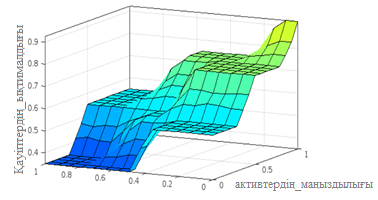
\includegraphics[width=0.8\textwidth]{media/ict/image27}
	\caption*{}
\end{figure}


а б

\begin{figure}[H]
	\centering
	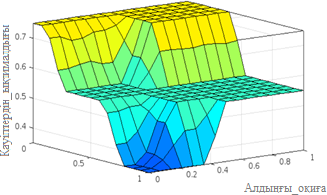
\includegraphics[width=0.8\textwidth]{media/ict/image29}
	\caption*{}
\end{figure}


в г

а - активтердің тартымдылығы және қолданыстағы бақылау туралы; б -
бұрынғы қауіптерден және активтердің тартымдылығынан; в - бұрынғы
қауіптерден және бар бақылаудан; г - келтірілген зиян деңгейінің
қаржылық шығындарға және беделге нұқсан келтіруге тәуелділігі

{\bfseries 2 - сурет. Қауіптердің ықтималдығының тәуелділігі}

{\bfseries Нәтижелер және талқылау.} Анық емес жиындар теориясы мен Мамдани
моделіне негізделген IIoT жүйелерінің ақпараттық қауіпсіздік
тәуекелдерін бағалаудың әзірленген моделі өнеркәсіптік IoT жүйелеріне
тән жоғары дәрежедегі белгісіздік жағдайында өзінің тиімділігін
көрсетті. Зерттеудің негізгі мақсаты компоненттердің өзара байланысының
жоғары дәрежесі, құрылымның күрделілігі мен қажеттілігі сияқты
өнеркәсіптік заттар интернетінің спецификалық ерекшеліктерін ескеретін
ақпараттық қауіпсіздік тәуекелдерін бағалаудың практикалық құралын жасау
болды. маңызды жүйелердің үздіксіз жұмысын қамтамасыз ету.

Осы жұмыстың нәтижелерін басқа зерттеулердің нәтижелерімен салыстыру
анық емес жиындар теориясын пайдалану әсіресе жоғары белгісіздік
жағдайында тәуекелді бағалаудың жоғары дәлдігін қамтамасыз ететінін
көрсетеді. Мысалы, ISO/IEC 27005 стандартында сипатталған тәуекелді
бағалау әдістемесі тәуекелді сапалы бағалауға ерекше мән береді, бірақ
белгісіздік жағдайында сандық талдау үшін құралдарды қамтамасыз етпейді.
Керісінше, ұсынылған модель әртүрлі кибершабуыл сценарийлерін есепке
алуға және сандық көрсеткіштерді пайдалана отырып ықтимал салдарларды
болжауға мүмкіндік береді.

Сонымен қатар, жақсы анықталған ықтималдықтарға негізделген дәстүрлі
әдістермен салыстырғанда (мысалы, NIST SP 800-39) әзірленген модель
толық емес немесе нақты емес ақпаратты қамтитын деректерді өңдеуде үлкен
икемділікті қамтамасыз етеді. Бұл деректер әртүрлі көздерден, соның
ішінде сенсорлардан, контроллерлерден және бұлттық платформалардан
алынатын, қателер мен белгісіздік ықтималдығын арттыратын IIoT жүйелері
үшін өте маңызды.

{\bfseries Қорытынды}. Мақала өнеркәсіптік IoT жүйелеріндегі ақпараттық
қауіпсіздік қатерлерді талдау мәселесін шешуге арналған. Бұл мәселені
шешу үшін анық емес логикалық әдістер қолданылды, өйткені дәл осы тәсіл
ақпаратта маңызды болып табылатын бағалаудың субъективтілігі болған
жағдайда, толық емес және дәл емес ақпарат жағдайында әртүрлі жүйелердің
жұмысын жақсарту мәселелерін шешуге мүмкіндік береді. қауіпсіздік.

Ұсынылған модель ақпараттық қауіпсіздік тәуекелдерін бағалау үшін
пайдаланылуы мүмкін, оны киберқауіпсіздік мамандары орындауы керек. Бұл
тәуекелдерді болжау және басымдық беру үшін пайдалы болуы мүмкін.
Сонымен қатар, ол тәуекелдерді бақылау және жүйелердің ақпараттық
қауіпсіздігін жақсарту бойынша шараларды жүзеге асыру саласындағы
маңызды ақпаратты ұсынады.

{\bfseries Әдебиеттер}

1. Hofer F. Architecture, technologies and challenges for cyber-physical
systems in industry 4.0: A systematic mapping study // 12th ACM/IEEE
internat. symp. Empirical Softw. Eng. Meas. -- NY., 2018. -- P. 1-10.
\href{https://doi.org/10.1145/3239235.3239242}{DOI
10.1145/3239235.3239242}

2. Sisinni E., Saifullah A., Han S. Industrial Internet of Things:
Challenges, opportunities, and directions // IEEE Trans. Ind. Informat.-
2018.-Vol.14(1) - P.4724-4734.

DOI
\href{https://doi.org/10.1109/TII.2018.2852491}{10.1109/TII.2018.2852491}

3. Tange K., De Donno M., Fafoutis X. et al. Systematic Survey of
Industrial Internet of Things Security: Requirements and Fog Computing
Opportunities // IEEE Communications Surveys \& Tutorials.- 2020.- Vol.
22(1). - P.2489-2520. DOI
\href{http://dx.doi.org/10.1109/COMST.2020.3011208}{10.1109/COMST.2020.3011208}

4. Yu X., Guo H. A Survey on IIoT Security // Procced. IEEE VTS Asia
Pacific Wireless Communications sympos//Singaporeю- 2019. -P.1-5 DOI
10.1109/VTS-APWCS.2019.8851679

5. Panchal A., Khadse V., Mahalle P. Security Issues in IIoT: A
Comprehensive Survey of Attacks on IIoT and Its Countermeasures //
Procced. 2018 IEEE Global conf. on Wireless Computing and Networking
(GCWCN).- Lonavala.- 2018.-P.124-130 DOI 10.1109/GCWCN.2018.8668630

6. Shah Y., Sengupta S. A survey on Classification of Cyber-attacks on
IoT and IIoT devices // Procced. 2020 11th IEEE Annual Ubiquitous
Computing, Electronics \& Mobile Communication conf. (UEMCON).- NY.-
2020. - P. 406-413.DOI 10.1109/UEMCON5185.2020.9298138

7. Hassani H. Vulnerability and security risk assessment in a IIoT
environment in compliance with standard IEC 62443 // Procedia Comput.
Sci.-2021.-№191.-Р. 33-40.

DOI 10.1016/j.procs.2021.07.008

8. Saaty T. What is the Analytic Hierarchy Process? // Mathematical
Models for Decision Support. -1988.-Vol.48. - P. 109-121. DOI
10.1007/978-3-642-83555-1\_5

9. Курейчик В.М. Особенности построения систем поддержки принятия
решений // Известия ЮФУ. Технические науки.- 2012. -№7(132). - С. 92-98.

10. Ani U., Tiwari A. Review of cybersecurity issues in industrial
critical infrastructure: manufacturing in perspective // Journal of
Cyber Security Technology.-2017.-Vol.1(1).- P. 32-74. DOI
10.1080/23742917.2016.1252211

11. Новак В., Перфильева И.Г., Мочкорж И. Математические принципы
нечеткой логики. -- М.: Физматлит, 2006. - 352 с. ISBN: 5-9221-0399-7

12. Абалдова С.Ю., Волынский В.Ю. Разработка системы нечеткого вывода
оценки результативности системы менеджмента качества предприятия на
основе алгоритма Мамдани // Известия высших учебных заведений. Серия:
Экономика, финансы и управление производством.- 2011. - №1.- С.86-93.

13. Голосовский М.С., Богомолов А.В., Теребов Д.С. и др. Алгоритм
настройки системы нечёткого логического вывода типа Мамдани // Вестник
Южно-Уральского государственного университета. - 2018. - № 3. - С.
19-29. DOI 10.14529/mmph180303

14. Горбачев С.В. Фаззификация экспертных лингвистических данных,
заданных в порядковой шкале // Матер. докл. 4-й междунар. заочн.
Науч.-практ. конф. «Интеллектуальные информационные системы: тенденции,
проблемы, перспективы (ИИС-2016). - Курск, 2017.- С. 47-49.

15. Belarbi K. Design of Mamdani fuzzy logic controllers with rule base
minimisation using genetic algorithm // Engineering applications of
artificial intelligence. - 2005.-Vol.18(7). - P. 875-880. DOI
10.1016/j.engappai.2005.03.003

16. Амирова А.С., Тохметов А.Т., Жанасбаева А.С. Основные проблемы
безопасности в промышленном интернете вещей // Вестник
Восточно-Казахстанского технического университета им. Д.Серикбаева. -
2021.- №1(91). -С. 82-91.

DOI 10.51885/1561-4212\_2021\_1\_82

17. Грибин М.А. Применение алгоритма Мамдани в системах автоматического
управления // Развитие современной науки: теоретические и прикладные
аспекты. -2019.- № 22. - С. 16-19.

18. ISO/IEC 27001:2022. Информационная безопасность, кибербезопасность и
защита персональных данных. URL:
https://pqm-online.com/assets/files/pubs/translations/std/iso-mek-27001-2022.pdf.
Дата обращения: 14.12.2024.

19. ISO/IEC 27005:2022. Information security, cybersecurity and privacy
protection. URL: https://www.iso.org/standard/80585. Date of address:
14.12.2024.

20. NIST SP 800-39. Managing Information Security Risk. URL:
https://nvlpubs.nist.gov/nistpubs/Legacy/SP/nistspecialpublication. Date
of address: 14.12.2024.

21. Методология FAIR (Factor Analysis of Information Risk). URL:
\url{https://www.risklens.com/hubfs/u}
ploads/2019/04/An\_Adoption\_Guide. Date of address:

14.12.2022.

22. Методология OCTAVE для оценки информационных рисков. URL:
http://www.risk24.ru/octave.htm. Дата обращения:14.12.2022.

23. Amirova A., Tokhmetov A. A model for risk analysis in the industrial
internet of things // Journal of Theoretical and Applied Information
Technology. -2021.- Vol.99(14). - P. 3449-3459.

24. Kerimkhulle S., Dildebayeva Zh., Tokhmetov А., Amirova А., Tussupov
J., Makhazhanova U., Adalbek А., Taberkhan R., Zakirova А., Salykbayeva
А. Fuzzy Logic and Its Application in the Assessment of Information
Security Risk of Industrial Internet of Things // Symmetry. -- 2023.
--Vol.15(10) - Р. 1-29. DOI10.3390/sym15101958

{\bfseries References}

1. Hofer F. Architecture, technologies and challenges for cyber-physical
systems in industry 4.0: A systematic mapping study // 12th ACM/IEEE
internat. symp. Empirical Softw. Eng. Meas. -- NY., 2018. -- P. 1-10.
\href{https://doi.org/10.1145/3239235.3239242}{DOI
10.1145/3239235.3239242}

2. Sisinni E., Saifullah A., Han S. Industrial Internet of Things:
Challenges, opportunities, and directions // IEEE Trans. Ind. Informat.-
2018.-Vol.14(1) - P.4724-4734.

DOI
\href{https://doi.org/10.1109/TII.2018.2852491}{10.1109/TII.2018.2852491}

3. Tange K., De Donno M., Fafoutis X. et al. Systematic Survey of
Industrial Internet of Things Security: Requirements and Fog Computing
Opportunities // IEEE Communications Surveys \& Tutorials.- 2020.- Vol.
22(1). - P.2489-2520. DOI
\href{http://dx.doi.org/10.1109/COMST.2020.3011208}{10.1109/COMST.2020.3011208}

4. Yu X., Guo H. A Survey on IIoT Security // Procced. IEEE VTS Asia
Pacific Wireless Communications sympos//Singaporeю- 2019. -P.1-5 DOI
10.1109/VTS-APWCS.2019.8851679

5. Panchal A., Khadse V., Mahalle P. Security Issues in IIoT: A
Comprehensive Survey of Attacks on IIoT and Its Countermeasures //
Procced. 2018 IEEE Global conf. on Wireless Computing and Networking
(GCWCN).- Lonavala.- 2018.-P.124-130 DOI 10.1109/GCWCN.2018.8668630

6. Shah Y., Sengupta S. A survey on Classification of Cyber-attacks on
IoT and IIoT devices // Procced. 2020 11th IEEE Annual Ubiquitous
Computing, Electronics \& Mobile Communication conf. (UEMCON).- NY.-
2020. - P. 406-413.DOI 10.1109/UEMCON5185.2020.9298138

7. Hassani H. Vulnerability and security risk assessment in a IIoT
environment in compliance with standard IEC 62443 // Procedia Comput.
Sci.-2021.-№191.-Р. 33-40.

DOI 10.1016/j.procs.2021.07.008

8. Saaty T. What is the Analytic Hierarchy Process? // Mathematical
Models for Decision Support. -1988.-Vol.48. - P. 109-121. DOI
10.1007/978-3-642-83555-1\_5

9. Kurejchik V.M. Osobennosti postroenija sistem podderzhki prinjatija
reshenij // Izvestija JuFU. Tehnicheskie nauki.- 2012. -№7(132). - S.
92-98.{[}in Russian{]}

10. Ani U., Tiwari A. Review of cybersecurity issues in industrial
critical infrastructure: manufacturing in perspective // Journal of
Cyber Security Technology.-2017.-Vol.1(1).- P. 32-74. DOI
10.1080/23742917.2016.1252211

11. Novak V., Perfil' eva I.G., Mochkorzh I.
Matematicheskie principy nechetkoj logiki. -- M.: Fizmatlit, 2006. - 352
s. ISBN: 5-9221-0399-7.{[}in Russian{]}

12. Abaldova S.Ju., Volynskij V.Ju. Razrabotka sistemy nechetkogo vyvoda
ocenki rezul' tativnosti sistemy menedzhmenta kachestva
predprijatija na osnove algoritma Mamdani // Izvestija vysshih uchebnyh
zavedenij. Serija: Jekonomika, finansy i upravlenie proizvodstvom.-
2011. - №1.- S.86-93. {[}in Russian{]}

13. Golosovskij M.S., Bogomolov A.V., Terebov D.S. i dr. Algoritm
nastrojki sistemy nechjotkogo logicheskogo vyvoda tipa Mamdani //
Vestnik Juzhno-Ural' skogo gosudarstvennogo universiteta.
- 2018. - № 3. - S. 19-29. DOI 10.14529/mmph180303.{[}in Russian{]}

14. Gorbachev S.V. Fazzifikacija jekspertnyh lingvisticheskih dannyh,
zadannyh v porjadkovoj shkale // Mater. dokl. 4-j mezhdunar. zaochn.
Nauch.-prakt. konf. «Intellektual' nye informacionnye
sistemy: tendencii, problemy, perspektivy (IIS-2016). - Kursk, 2017.- S.
47-49. {[}in Russian{]}

15. Belarbi K. Design of Mamdani fuzzy logic controllers with rule base
minimisation using genetic algorithm // Engineering applications of
artificial intelligence. - 2005.-Vol.18(7). - P. 875-880. DOI
10.1016/j.engappai.2005.03.003

16. Amirova A.S., Tohmetov A.T., Zhanasbaeva A.S. Osnovnye problemy
bezopasnosti v promyshlennom internete veshhej // Vestnik
Vostochno-Kazahstanskogo tehnicheskogo universiteta im. D.Serikbaeva. -
2021.- №1(91). -S. 82-91. {[}in Russian{]}

DOI 10.51885/1561-4212\_2021\_1\_82

17. Gribin M.A. Primenenie algoritma Mamdani v sistemah avtomaticheskogo
upravlenija // Razvitie sovremennoj nauki: teoreticheskie i prikladnye
aspekty. -2019.- № 22. - S. 16-19. {[}in Russian{]}

18. ISO/IEC 27001:2022. Informacionnaja bezopasnost',
kiberbezopasnost'{} i zashhita
personal' nyh dannyh. URL:
https://pqm-online.com/assets/files/pubs/translations/std/iso-mek-27001-2022.pdf.
Data obrashhenija: 14.12.2024. {[}in Russian{]}

19. ISO/IEC 27005:2022. Information security, cybersecurity and privacy
protection. URL: https://www.iso.org/standard/80585. Date of address:
14.12.2024.

20. NIST SP 800-39. Managing Information Security Risk. URL:
https://nvlpubs.nist.gov/nistpubs/Legacy/SP/nistspecialpublication. Date
of address: 14.12.2024.

21. Metodologija FAIR (Factor Analysis of Information Risk). URL:
\url{https://www.risklens.com/hubfs/u}
ploads/2019/04/An\_Adoption\_Guide. Date of address:

14.12.2022. {[}in Russian{]}

22. Metodologija OCTAVE dlja ocenki informacionnyh riskov. URL:
http://www.risk24.ru/octave.htm. Data obrashhenija:14.12.2022. {[}in
Russian{]}

23. Amirova A., Tokhmetov A. A model for risk analysis in the industrial
internet of things // Journal of Theoretical and Applied Information
Technology. -2021.- Vol.99(14). - P. 3449-3459.

24. Kerimkhulle S., Dildebayeva Zh., Tokhmetov А., Amirova А., Tussupov
J., Makhazhanova U., Adalbek А., Taberkhan R., Zakirova А., Salykbayeva
А. Fuzzy Logic and Its Application in the Assessment of Information
Security Risk of Industrial Internet of Things // Symmetry. -- 2023.
--Vol.15(10) - Р. 1-29. DOI10.3390/sym15101958

\emph{{\bfseries Сведения об авторах}}

Амирова А.С. - PhD, ассистент профессор, Astana IT University, Астана,
Казахстан, e-mail:
\href{mailto:akzhibek.amirova@astanait.edu.kz}{\nolinkurl{akzhibek.amirova@astanait.edu.kz}};

Құттыбек А.А. -- сеньор-лектор, Astana IT University, Астана, Казахстан,
e-mail:
\href{mailto:azhar.kuttybek@astanait.edu.kz}{\nolinkurl{azhar.kuttybek@astanait.edu.kz}};

Есмагамбетова М.М.- PhD, доцент - Карагандинский университет
Казпотребсоюза, Караганда, Казахстан e-mail:
\href{mailto:marzhan1983@mail.ru}{\nolinkurl{marzhan1983@mail.ru}};

Есмагамбетов Т.У.- магистр, старший преподаватель - Карагандинский
университет Казпотребсоюза, Караганда, Казахстан e-mail:
\href{mailto:Timur198300@mail.ru}{\nolinkurl{Timur198300@mail.ru}}

\emph{{\bfseries Information about the authors}}

Amirova A.S. - PhD, assistant professor, Astana IT University, Astana,
Kazakhstan, e-mail:
\href{mailto:akzhibek.amirova@astanait.edu.kz}{\nolinkurl{akzhibek.amirova@astanait.edu.kz}};

Kuttybek A.A. -- senior lecturer, Astana IT University, Astana,
Kazakhstan, e-mail:
\href{mailto:azhar.kuttybek@astanait.edu.kz}{\nolinkurl{azhar.kuttybek@astanait.edu.kz}};

Yesmagambetova M.M.- PhD, assistant professor, Karaganda University of
Kazpotrebsoyuz, Karaganda, Kazakhstan e-mail:
\href{mailto:marzhan1983@mail.ru}{\nolinkurl{marzhan1983@mail.ru}};

Yesmagambetov T.U.- master, senior lecturer, Karaganda University of
Kazpotrebsoyuz, Karaganda, Kazakhstan e-mail:
\href{mailto:Timur198300@mail.ru}{\nolinkurl{Timur198300@mail.ru}};

ГРНТИ 28.23.15

{\bfseries RECOGNITION OF PLANT DISEASES FROM LEAF IMAGES USING MACHINE}

{\bfseries LEARNING TECHNOLOGY}

{\bfseries \textsuperscript{1}N.
\begin{figure}[H]
	\centering
	
\includegraphics[width=0.8\textwidth]{media/ict/image1}
	\caption*{}
\end{figure}

\textsuperscript{2}Sh.
\begin{figure}[H]
	\centering
	
\includegraphics[width=0.8\textwidth]{media/ict/image1}
	\caption*{}
\end{figure}

\textsuperscript{2}A.
\begin{figure}[H]
	\centering
	
\includegraphics[width=0.8\textwidth]{media/ict/image1}
	\caption*{}
\end{figure}

\textsuperscript{3}K.
\begin{figure}[H]
	\centering
	
\includegraphics[width=0.8\textwidth]{media/ict/image1}
	\caption*{}
\end{figure}


{\bfseries \textsuperscript{3}A.
\begin{figure}[H]
	\centering
	
\includegraphics[width=0.8\textwidth]{media/ict/image1}
	\caption*{}
\end{figure}


\emph{\textsuperscript{1}K. Kulazhanov Kazakh University of Technology
and Business, Astana, Kazakhstan,}

\emph{\textsuperscript{2}Taraz Regional University named after
M.KH.Dulaty, Taraz, Kazakhstan,}

\emph{\textsuperscript{3}L.N. Gumilyov Eurasian National University,
Astana, Kazakhstan}

{\bfseries \textsuperscript{\envelope }}Correspondent-author\emph{:}
\href{mailto:yaphets9705@gmail.com}{\nolinkurl{yaphets9705@gmail.com}}

This article presents a Python-oriented solution for automatic
classification of plants based on image analysis, applicable in
agriculture, ecology and botany. Traditional plant identification
methods, which require expert analysis, are often time-consuming and
error-prone. The developed application uses convolutional neural
networks (CNN) implemented on the basis of TensorFlow to recognize
plants by their visual characteristics, which allows you to accurately
and quickly classify species. An important role is played by the OpenCV
library, which is used for image preprocessing, including resizing,
color normalization and noise filtering, which improves classification
accuracy. The model achieves an accuracy of 86.97\%, which confirms its
effectiveness and suitability for practical use. The system is equipped
with an intuitive interface, which makes it accessible to users of
different levels of training. In the future, it is planned to expand the
functionality by increasing the database and introducing transfer
learning methods to improve accuracy.

{\bfseries Keywords:} plant classification, Python, TensorFlow, CNN,
OpenCV, machine learning, image processing.

{\bfseries РАСПОЗНАВАНИЕ БОЛЕЗНЕЙ РАСТЕНИЙ ПО ИЗОБРАЖЕНИЯМ ЛИСТЬЕВ С
ИСПОЛЬЗОВАНИЕМ ТЕХНОЛОГИИ МАШИННОГО ОБУЧЕНИЯ}

{\bfseries \textsuperscript{1}Н.Ә. Жұматай, \textsuperscript{2}Ш.Е.
Ахметжанова, \textsuperscript{2}А.Д. Абдувалова, \textsuperscript{3}К.Ш.
Бейсенбаева, \textsuperscript{3}А.Жанарбекұлы\textsuperscript{\envelope }}

\emph{\textsuperscript{1}Казахский университет технологии и бизнеса им.
К. Кулажанова, Астана, Казахстан,}

\emph{\textsuperscript{2}Таразский региональный университет им.М. Х.
Дулати, Тараз, Казахстан,}

\emph{\textsuperscript{3}Евразийский национальный университет имени
Л.Н.Гумилева, Астана, Казахстан,}

\emph{e-mail:\href{mailto:yaphets9705@gmail.com}{\nolinkurl{yaphets9705@gmail.com}}}

Данная статья представляет Python-ориентированное решение для
автоматической классификации растений на основе анализа изображений,
применимое в сельском хозяйстве, экологии и ботанике. Традиционные
методы идентификации растений, требующие экспертного анализа, часто
отнимают много времени и подвержены ошибкам. Разработанное приложение
использует свёрточные нейронные сети (CNN), реализованные на базе
TensorFlow, для распознавания растений по их визуальным признакам, что
позволяет точно и быстро классифицировать виды. Важную роль играет
библиотека OpenCV, используемая для предварительной обработки
изображений, включающей изменение размеров, нормализацию цвета и
фильтрацию шумов, что повышает точность классификации. Модель достигает
точности 86.97\%, что подтверждает её эффективность и пригодность для
практического применения. Система оснащена интуитивно понятным
интерфейсом, что делает её доступной для пользователей разного уровня
подготовки. В будущем планируется расширение функционала за счёт
увеличения базы данных и внедрения методов трансферного обучения для
улучшения точности.

{\bfseries Ключевые слова:} классификация растений, Python, TensorFlow,
CNN, OpenCV, машинное обучение, обработка изображений.

{\bfseries МАШИНАЛЫҚ ОҚЫТУ ТЕХНОЛОГИЯСЫН ҚОЛДАНА ОТЫРЫП, ЖАПЫРАҚ КЕСКІНДЕРІ
АРҚЫЛЫ ӨСІМДІК АУРУЛАРЫН ТАНУ}

{\bfseries \textsuperscript{1}Н.Ә. Жұматай, \textsuperscript{2}Ш.Е.
Ахметжанова, \textsuperscript{2}А.Д. Абдувалова, \textsuperscript{3}К.Ш.
Бейсенбаева, \textsuperscript{3}А.Жанарбекұлы\textsuperscript{\envelope }}

\emph{{\bfseries \textsuperscript{1}}Қ. Құлажанов атындағы Қазақ технология
және бизнес университеті, Астана қ., Қазақстан,}

\emph{\textsuperscript{2}М.Х.Дулати атындағы Тараз өңірлік университеті,
Тараз қ., Қазақстан,}

\emph{\textsuperscript{3}Л.Н.Гумилев атындағы Еуразия ұлттық
университеті, Астана қ., Қазақстан,}

\emph{e-mail:\href{mailto:yaphets9705@gmail.com}{\nolinkurl{yaphets9705@gmail.com}}}

Бұл мақала ауыл шаруашылығында, экологияда және ботаникада қолданылатын
кескінді талдау негізінде өсімдіктерді автоматты түрде жіктеуге арналған
Python-бағытталған шешімді ұсынады. Сараптамалық талдауды қажет ететін
өсімдіктерді анықтаудың дәстүрлі әдістері көбінесе көп уақытты қажет
етеді және қателіктерге бейім. Әзірленген қолданба өсімдіктерді визуалды
белгілері бойынша тану үшін TensorFlow негізіндегі конволюциялық
нейрондық желілерді (CNN) пайдаланады, бұл түрлерді дәл және жылдам
жіктеуге мүмкіндік береді. Өлшемін Өзгертуді, түсін қалыпқа келтіруді
және шуды сүзуді қамтитын кескіндерді алдын ала өңдеу үшін
пайдаланылатын OpenCV кітапханасы маңызды рөл атқарады, бұл жіктеу
дәлдігін арттырады. Модель 86.97\% дәлдікке жетеді, бұл оның тиімділігі
мен практикалық қолдануға жарамдылығын растайды. Жүйе интуитивті
интерфейспен жабдықталған, бұл оны әртүрлі деңгейдегі пайдаланушылар
үшін қол жетімді етеді. Болашақта деректер базасын ұлғайту және дәлдікті
жақсарту үшін трансферлік оқыту әдістерін енгізу есебінен
функционалдылықты кеңейту жоспарлануда.

{\bfseries Кілт сөздер:} өсімдіктерді жіктеу, Python, TensorFlow, CNN,
OpenCV, Машиналық оқыту, кескінді өңдеу.

{\bfseries Introduction.} The rapid advancement of image recognition
technology has paved the way for innovative applications across various
fields, including agriculture, ecology, and environmental sciences.
Accurate identification of plant species is a fundamental task in these
fields, aiding in biodiversity studies, conservation efforts, and pest
management. Traditional plant identification methods, relying on manual
classification by experts, are often time-consuming and prone to human
error. Automated plant identification systems, leveraging machine
learning and computer vision, provide a scalable and efficient
alternative to these traditional approaches.

This paper presents a Python-based application designed to classify
plant species from user-inputted images. Utilizing convolutional neural
networks (CNNs) for feature extraction and classification, the model
demonstrates an effective approach to recognizing plants based on visual
characteristics. The application is equipped with a user-friendly
interface, allowing users to submit an image for analysis, with the
model subsequently returning a probable plant species as output.

The objectives of this study include developing a robust preprocessing
pipeline to optimize image quality, selecting an appropriate model
architecture for high classification accuracy, and evaluating the
model' s performance against existing plant databases. By
leveraging modern machine learning frameworks and image processing
techniques, this research seeks to contribute a practical tool for
botanists, researchers, and agriculturalists in the pursuit of reliable
and scalable plant identification solutions.

{\bfseries Materials and methods. \emph{Overview of Python and Libraries
for Image Processing and Machine Learning}}

Python is widely recognized for its versatility and ease of use, making
it the preferred language for scientific and machine learning
applications. Its expansive ecosystem includes numerous libraries that
support high-performance computing, data analysis, and machine learning,
which are essential in building efficient applications for image
recognition tasks. In the domain of plant identification, Python enables
complex neural network architectures and image preprocessing
capabilities, which are fundamental to accurately distinguishing between
species based on visual data {[}1{]}.

TensorFlow, an open-source machine learning library developed by Google,
is instrumental in building and deploying machine learning models. Its
flexible architecture allows for the deployment of models across
multiple CPUs and GPUs, making it highly efficient for training large
datasets {[}2{]}. TensorFlow's Keras API is particularly useful for
developing deep learning models like Convolutional Neural Networks
(CNNs). CNNs are known for their ability to process and learn from
images by identifying spatial hierarchies of features, such as shapes,
textures, and edges, which are critical for distinguishing between
different plant species. CNNs achieve this by progressively extracting
feature maps from images, making them ideal for tasks that require
detailed visual analysis, such as plant disease classification {[}3{]}.

The use of TensorFlow also allows for implementing transfer learning,
where pre-trained models (such as InceptionV3, ResNet, or VGG16) are
fine-tuned on a specific dataset. Transfer learning greatly reduces
training time and improves model accuracy by leveraging patterns learned
from vast image datasets, which are applicable across various domains
{[}4{]}. This capability makes TensorFlow a powerful tool in developing
reliable models for plant identification.

OpenCV (Open Source Computer Vision Library) is an open-source library
designed to support real-time computer vision and image processing
tasks. OpenCV offers a wide array of tools for manipulating images, such
as resizing, filtering, and color adjustments, which are crucial steps
in preparing images for machine learning models {[}5{]}. For example,
resizing images to a standard input size improves consistency in model
training, while color normalization adjusts variations in lighting
conditions, reducing the influence of environmental factors on
classification accuracy {[}6{]}.

Additionally, OpenCV includes advanced filtering and edge-detection
techniques such as GaussianBlur, Canny Edge Detection, and Morphological
Transformations, which enhance features and reduce noise in images.
These techniques are particularly beneficial in plant identification,
where clarity of leaf texture, edges, and shape are essential for
accurate classification {[}7{]}.

By leveraging both TensorFlow and OpenCV, Python provides a cohesive
platform to manage the entire image classification pipeline, from data
preprocessing to model training and deployment. The use of these
libraries enables the creation of highly accurate plant identification
systems that can efficiently handle real-world variations in plant
appearance. The synergy between machine learning and image processing in
Python not only increases the model's accuracy but also optimizes
computational resources, making Python an ideal choice for plant
recognition tasks {[}8{]}.

Python's supportive community and comprehensive documentation for
libraries such as TensorFlow and OpenCV make it accessible even for
researchers with limited programming backgrounds. This accessibility,
coupled with the flexibility of Python' s ecosystem,
continues to drive its popularity in the scientific and machine learning
communities.

\emph{{\bfseries Process Flow Diagram Description.}} The following diagram
illustrates the workflow of the plant identification program, detailing
each step from user input to the final result display.

This structured approach ensures accurate classification of the plant
species based on the input image (Figure --1 ).

\begin{figure}[H]
	\centering
	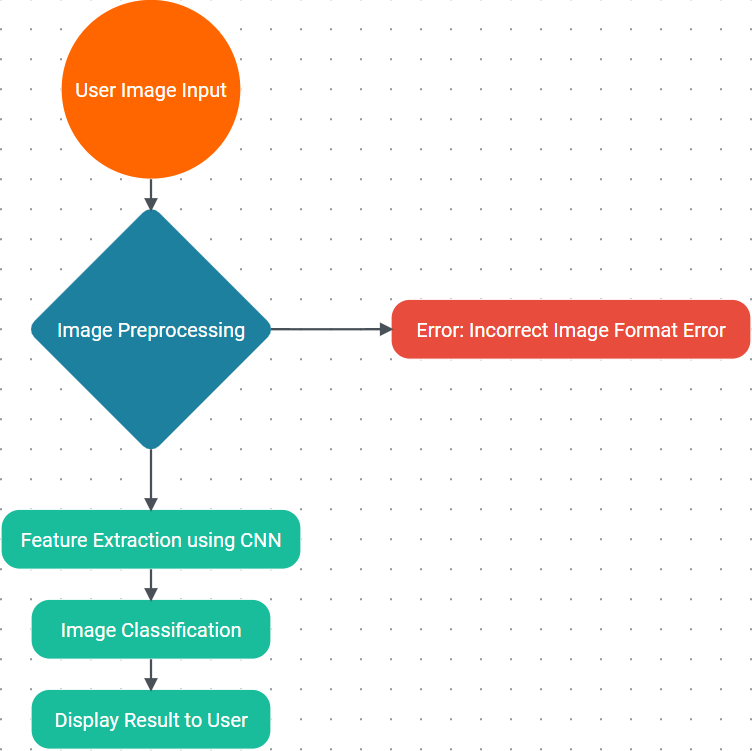
\includegraphics[width=0.8\textwidth]{media/ict/image31}
	\caption*{}
\end{figure}


Fig. 1 - Workflow of the plant identification program

The process of plant identification begins with the user uploading an
image of a plant. This image can depict various parts of the plant,
including leaves, flowers, or the entire plant itself. It serves as the
primary input data for the program. For accurate processing, it is
crucial that the uploaded image conforms to specific requirements in
terms of format and resolution. Common formats accepted by the program
typically include JPEG, PNG, and BMP. The resolution of the image should
be sufficient to capture the details necessary for effective
analysis---ideally, the dimensions should not be less than 224x224
pixels to ensure clarity during feature extraction.

Upon receiving the image, the program utilizes the OpenCV library, a
powerful tool for image processing and computer vision tasks. The
preprocessing phase is critical, as it enhances the image quality and
optimizes the performance of the machine learning model.

During this stage, the program first checks the uploaded image for
correctness in format. If the image format does not meet the accepted
criteria, an error message---"Incorrect Image Format Error"---is
displayed. This prompt guides the user to upload a compatible file,
ensuring that the input data is valid before proceeding further.

Resizing: The image is resized to specified dimensions (commonly 224x224
pixels). This standardization is crucial to maintain consistency across
all inputs, which helps to avoid potential scaling issues that could
adversely affect classification accuracy.

Color Normalization: This step adjusts the image for variations in
lighting and shadows. Color normalization helps mitigate the influence
of external factors, such as differences in illumination or background
scenery, thereby creating a more uniform basis for analysis.

Noise Filtering: Noise can often obscure important features in an image,
so filtering techniques are applied to eliminate artifacts. Methods such
as Gaussian blur or median filtering are employed to smooth the image,
which enhances the model' s ability to detect relevant
features accurately.

Once the image preprocessing is complete, the preprocessed image is
passed to a Convolutional Neural Network (CNN) model, which is
implemented using TensorFlow. The CNN is designed to automatically
extract hierarchical features from the image. These features include
shapes, textures, and edges that are characteristic of different plant
species.

This feature extraction process is fundamental for the subsequent
classification task. By identifying and isolating unique features, the
CNN enables the model to differentiate between various species of
plants. Each layer of the CNN extracts increasingly complex features,
allowing for a deep understanding of the visual data presented in the
image.

After feature extraction, the CNN analyzes the gathered features and
classifies the image based on their correlations with specific plant
types. The model calculates probabilities for each potential class
(plant species) and selects the class with the highest probability as
the final classification result.

For instance, if the model analyzes an image of a plant and identifies
key features indicative of lavender, it may conclude that the image
corresponds to the ``Lavender'' class with a confidence level of 90\%.
This confidence score reflects the model's certainty about its
classification, which is critical for user trust and usability.

Once the classification is complete, the program displays the results to
the user. This output includes the name of the identified plant and may
also provide additional information, such as its scientific name, common
characteristics, or a brief description of its ecological significance.

In cases where the model' s confidence level is
low-indicating uncertainty about the classification-the program offers
additional guidance. The user might receive suggestions to upload a
clearer image or to try a different angle that better captures the
plant' s distinguishing features. This interactive
element not only improves the user experience but also enhances the
likelihood of obtaining accurate results in subsequent attempts.

\emph{{\bfseries Image Preprocessing.}} Resizing is a fundamental
preprocessing step in image analysis, particularly for machine learning
applications. The process involves changing the dimensions of an image
to a standard size that is compatible with the model' s
input requirements. For example, many deep learning models, including
Convolutional Neural Networks (CNNs), often expect input images to be of
specific dimensions-commonly 224x224 pixels.

The importance of resizing lies in its ability to maintain consistency
across all images fed into the model. When images of varying sizes are
used, it can lead to discrepancies during feature extraction, making it
challenging for the model to learn effectively. Uniformity in size helps
in stabilizing the learning process, enabling the model to focus on the
actual features rather than adjusting to differences in image
dimensions. Additionally, resizing reduces the computational load,
allowing for faster processing and improved efficiency during training
and inference stages {[}9{]}.

Filtering techniques are employed to enhance image quality by reducing
noise and artifacts that can obscure significant features. Common
filtering methods include:

\begin{itemize}
\item
  Gaussian Blur: This technique smooths the image by averaging pixel
  values in a neighborhood defined by a Gaussian function. It helps in
  eliminating high-frequency noise and reduces detail in the image,
  which can otherwise interfere with the learning process. By
  suppressing noise, the model can better identify critical features
  that contribute to accurate classification {[}10{]}.
\item
  Median Filtering: Unlike Gaussian blur, median filtering replaces each
  pixel value with the median of the neighboring pixels. This method is
  particularly effective at removing salt-and-pepper noise while
  preserving edges, which are essential for accurate feature extraction.
  The preservation of edges aids the model in recognizing the contours
  and shapes that are characteristic of different plant species
  {[}11{]}.
\end{itemize}

By applying these filtering techniques, the preprocessing stage enhances
the clarity of the images, allowing the model to learn from more
representative data. A cleaner input leads to more reliable feature
extraction and ultimately contributes to improved classification
accuracy.

Normalization is a process that adjusts the pixel values of an image to
ensure consistent representation across different lighting conditions
and backgrounds. This method is crucial for reducing the impact of
variability in image acquisition, which can arise from different sources
of illumination or environmental conditions.

Color normalization techniques may involve transforming the
image' s color space (e.g., converting from RGB to HSV)
or adjusting pixel intensities to fit a specified range. This process
helps in balancing the overall brightness and contrast of the image,
enabling the model to focus on intrinsic features rather than extraneous
visual noise{[}12{]}.

Normalization plays a pivotal role in enhancing model accuracy by
ensuring that the neural network receives input data that is
representative of the actual features it needs to learn. By mitigating
the effects of inconsistent lighting and color variations, normalization
allows the model to generalize better from training data to unseen
instances, thereby improving its performance in real-world applications.

In summary, the preprocessing of images through resizing, filtering, and
normalization is critical for enhancing the accuracy of machine learning
models, especially in the context of plant identification. Each of these
techniques contributes to creating a more uniform and representative
dataset, which in turn enables the model to extract meaningful features
and make accurate classifications. The importance of these preprocessing
methods cannot be overstated, as they lay the groundwork for effective
learning and reliable performance in image classification tasks.

{\bfseries Results and discussion. \emph{Machine learning model for plant
disease classification}}

In the realm of agricultural technology, the ability to accurately
diagnose plant diseases is crucial for maintaining healthy crops and
ensuring food security. To achieve this, we developed a machine learning
model based on a Convolutional Neural Network (CNN) architecture,
specifically saved as cnn\_plant\_disease\_model.keras. CNNs are
particularly well-suited for image recognition tasks due to their
ability to automatically extract and learn features from images.

The CNN architecture utilized in this study comprises several
convolutional layers, each followed by activation functions and pooling
layers. This structure allows the model to learn hierarchical
representations of the input data, enabling it to capture intricate
details in plant images. By employing multiple layers, the CNN can
detect features ranging from simple edges and textures in the early
layers to complex patterns in the deeper layers.

For effective model training, a comprehensive dataset was essential. The
dataset consisted of thousands of images of various plant species, each
labeled with the corresponding disease status. The images were collected
from diverse sources to ensure variability in conditions, such as
lighting and angles, thus enhancing the model' s
robustness.

To further improve the model' s performance, data
augmentation techniques were applied. These techniques included random
rotations, zooming, flipping, and brightness adjustments. By
artificially increasing the diversity of the training dataset, we aimed
to help the model generalize better to unseen data, thereby reducing the
risk of overfitting.

Prior to training, all images underwent preprocessing to optimize them
for input into the CNN. The preprocessing steps included resizing images
to a standard dimension of 224x224 pixels and normalizing pixel values
to a range between 0 and 1. This standardization is vital for improving
the model' s convergence speed during training.

The model was trained using a robust dataset split into training and
validation sets, with 80\% of the data allocated for training and 20\%
for validation. The training process involved multiple epochs, with a
batch size of 32. This configuration allowed the model to learn from a
sufficient number of samples in each iteration while maintaining
efficient computational performance.

We employed the Adam optimizer, a popular choice in deep learning for
its adaptive learning rate capabilities. The loss function used was
categorical cross-entropy, suitable for multi-class classification
tasks. This combination of optimizer and loss function facilitated
efficient training and convergence of the model.

The "Training and validation accuracy over epochs" graph illustrates the
model' s performance in terms of accuracy throughout the
training process. On the X-axis, we have the number of Epochs, while the
Y-axis represents the Training Accuracy and Validation Accuracy Figure
-- 2).

\begin{figure}[H]
	\centering
	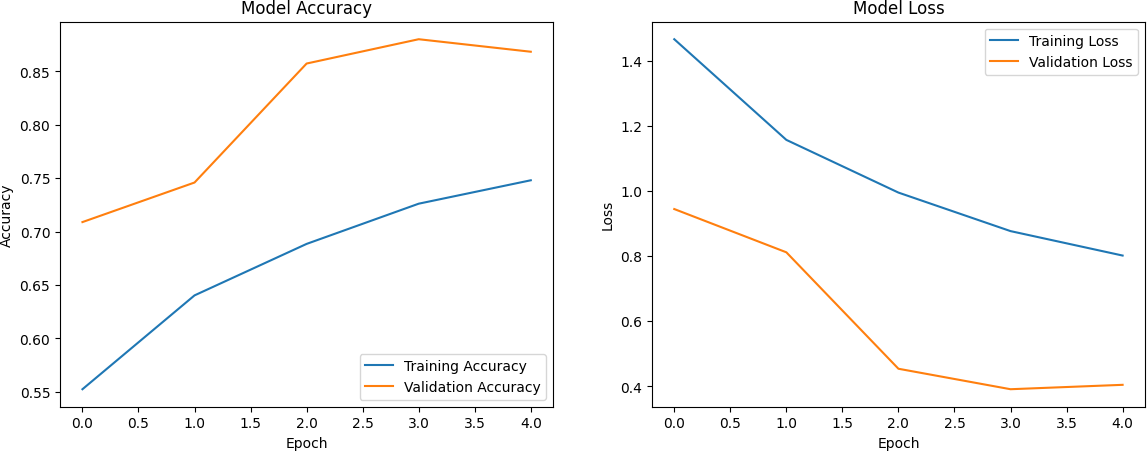
\includegraphics[width=0.8\textwidth]{media/ict/image32}
	\caption*{}
\end{figure}


Fig. 2 - Training and validation accuracy over epochs

As the training progresses through the epochs, we observe a significant
increase in both training and validation accuracy. Initially, the model
demonstrates relatively low accuracy, which gradually improves as it
learns from the training dataset. By the end of the training, the model
achieves an accuracy of 86.97\% (or 0.8697), indicating that it can
correctly classify the majority of plant images in the validation
dataset. This high accuracy reflects the model's effectiveness in
capturing the relevant features necessary for plant disease
classification.

The gap between training accuracy and validation accuracy should be
monitored closely. If the training accuracy is significantly higher than
the validation accuracy, it may indicate overfitting. However, in this
case, the model appears to maintain a good balance between the two,
suggesting effective generalization to unseen data.

The "Training and validation loss over epochs" graph presents the loss
values recorded throughout the training process. The X-axis represents
the number of Epochs, while the Y-axis displays the Training Loss and
Validation Loss (Figure - 3).

\begin{figure}[H]
	\centering
	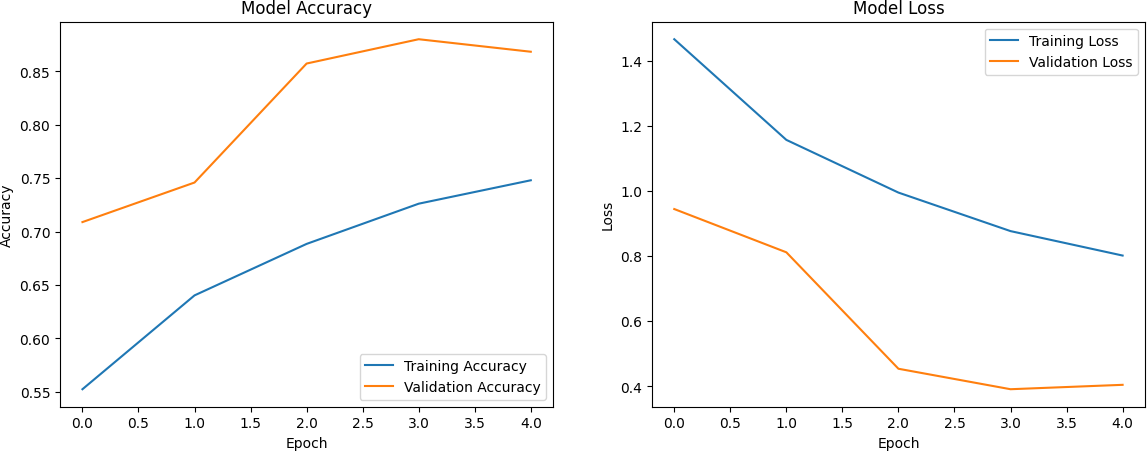
\includegraphics[width=0.8\textwidth]{media/ict/image32}
	\caption*{}
\end{figure}


Fig.3- Training and validation loss over epochs

Initially, both training and validation loss values are high, indicating
that the model' s predictions deviate significantly from
the actual labels. However, as training progresses, both loss values
decrease steadily. The Training Loss reaches a value of 0.4000,
demonstrating that the model' s predictions increasingly
align with the actual data as it learns. A lower loss value indicates a
better performance in classification tasks, suggesting that the model
has effectively minimized the error in its predictions.

The convergence of training and validation loss towards the end of the
training process further supports the model' s stability
and its capability to generalize well. If the validation loss starts to
increase while training loss continues to decrease, it would be a sign
of overfitting; however, this scenario is not observed in our results.

To illustrate the model' s performance, we generated
accuracy and loss curves during the training process. {[}Insert the
accuracy and loss graph here.{]} These visualizations depict the
model' s learning trajectory, showcasing how accuracy
improved and loss decreased over epochs. Observing these trends allows
us to assess the effectiveness of the training regimen.

The developed CNN model, cnn\_plant\_disease\_model.keras, holds
significant promise for practical applications in agriculture. By
enabling quick and accurate identification of plant diseases, this model
can assist farmers and agricultural specialists in making timely
decisions to manage crop health. This capability can ultimately lead to
improved yield and reduced economic losses due to disease outbreaks.

While the current model demonstrates commendable performance, several
avenues for future research exist. Exploring more advanced
architectures, such as deeper CNNs or transfer learning with pre-trained
models, could yield further improvements in accuracy. Additionally,
expanding the dataset to include more diverse plant species and diseases
would enhance the model' s applicability across different
agricultural contexts.

In summary, the CNN model developed for plant disease classification,
saved as cnn\_plant\_disease\_model.keras, achieved an impressive
accuracy of 86.97\% with a loss of 0.4000. This indicates a
well-optimized model capable of effectively identifying plant diseases
from images. As agricultural challenges continue to evolve, the
integration of machine learning technologies like this model offers
promising solutions for sustainable farming practices.

\emph{{\bfseries User interface and interaction in Plant disease
classification application.}} The plant disease classification
application is designed to provide a seamless user experience while
allowing users to accurately identify various plant species and diagnose
potential diseases.

The user interface (UI) is thoughtfully crafted to be intuitive,
facilitating easy navigation for individuals with varying levels of
technical expertise (Figure - 4).

\begin{figure}[H]
	\centering
	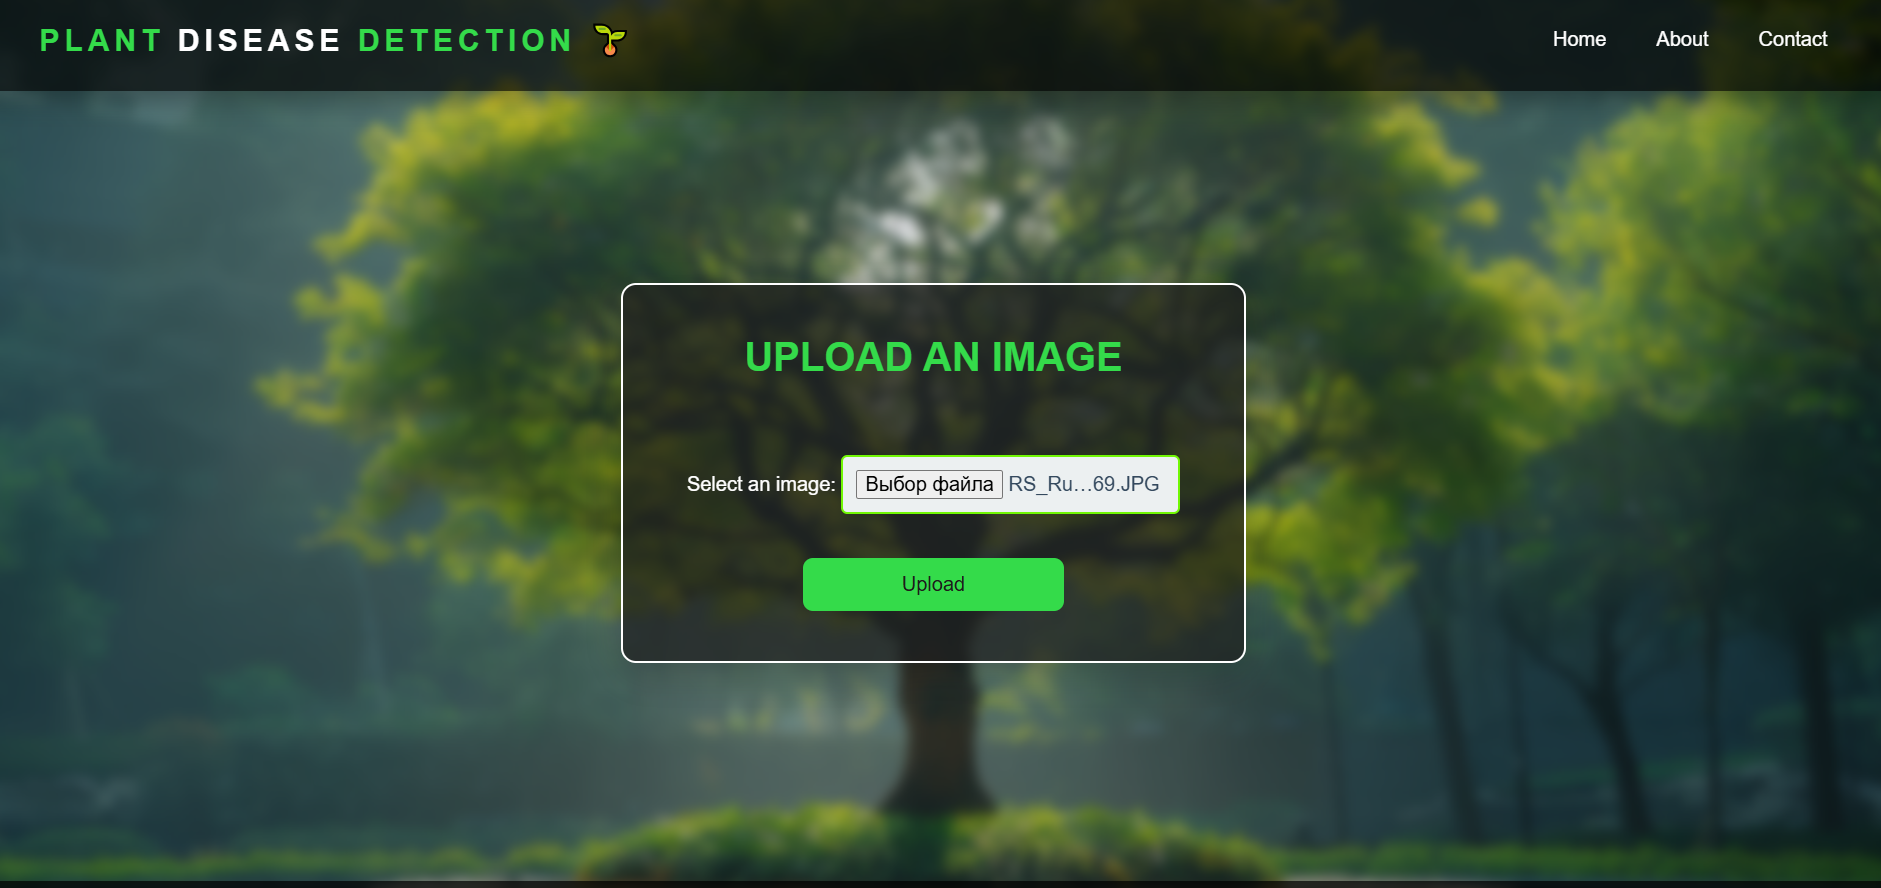
\includegraphics[width=0.8\textwidth]{media/ict/image33}
	\caption*{}
\end{figure}


Fig. 4 - Home page

The application guides users through a straightforward process,
beginning with the launch of the program on their device. Upon accessing
the main screen, users encounter a prominent prompt to upload an image
of a plant. This image can depict a leaf, flower, or the entire plant,
serving as the crucial input data for the classification model.

Users can initiate the process by clicking the "Upload Image" button,
which opens a file dialog for selecting an image. The application
supports multiple image formats, including JPEG, PNG, and BMP, ensuring
compatibility with commonly used files. Once an image is selected, the
program conducts a validation check to verify that the uploaded file
adheres to the necessary format and resolution specifications. If the
image format is deemed incorrect, the application promptly displays an
"Incorrect Image Format Error" message, guiding the user to upload a
compatible file.

After confirming the validity of the uploaded image, the program
utilizes the OpenCV library to preprocess the image. This stage includes
resizing, color normalization, and noise filtering, enhancing the image
quality for optimal performance of the model. A progress indicator may
appear during this phase, reassuring users that the processing is
underway. Upon completion of the image processing and classification,
the application presents the results prominently on the screen. Users
receive information about the identified plant species, including both
common and scientific names. Additionally, the program may provide
supplementary details, such as characteristics, potential diseases, and
care instructions.

The model' s confidence level in its classification is
also communicated to the user. For example, if the program identifies a
plant as ``Lavender'' with a confidence level of 90\%, this information
helps users assess the reliability of the result. Users are encouraged
to provide feedback on the classification results. If they believe the
classification is incorrect, they can submit their observations,
contributing to the model's continuous improvement.

To ensure a pleasant user experience, the interface incorporates several
interactive features. Accessibility features are designed with
inclusivity in mind, offering options such as screen reader
compatibility, text-to-speech for results, and adjustable font sizes to
cater to diverse user needs. A dedicated help section is available,
providing comprehensive information on how to navigate the application,
troubleshoot common issues, and interpret results. This resource is
particularly beneficial for first-time users unfamiliar with the
technology.

The option to create user profiles allows individuals to save uploaded
images and classification results for future reference. This feature is
advantageous for tracking the health of plants over time and comparing
different outcomes. The accuracy and performance of the plant disease
classification model are paramount to its usability. The model achieved
an accuracy of 86.97\% and a loss value of 0.4000 during training,
reflecting its capability to reliably classify a wide range of plant
species.

The accuracy of the model is determined by its ability to correctly
classify instances from a validation dataset. An accuracy of 86.97\%
signifies that the model can accurately identify the majority of plant
images, which is essential for practical applications in agriculture
where timely and precise diagnosis of plant diseases can significantly
impact crop management strategies. Beyond accuracy, additional
performance metrics such as precision, recall, and F1-score can be
computed to provide a more comprehensive understanding of the model's
performance. These metrics are particularly useful in scenarios where
class imbalances exist.

A confusion matrix can be generated to visualize the
model' s classification performance across various plant
species. This tool helps identify specific species that are frequently
misclassified, enabling targeted improvements in model performance. The
model has been trained to recognize a diverse array of plant species,
each exhibiting unique characteristics. For example, it can identify
Lavender (Lavandula angustifolia), known for its fragrant purple blooms,
which is commonly used in aromatherapy and culinary applications. The
model can accurately identify tomato plants (Solanum lycopersicum), a
widely cultivated vegetable, by their characteristic green foliage and
red fruits. It also recognizes roses (Rosa spp.), known for their
beauty, and corn (Zea mays), a staple crop identifiable by its tall
stalks and long, narrow leaves. Additionally, the model can recognize
basil (Ocimum basilicum), a popular culinary herb identifiable by its
broad, green leaves and aromatic scent.

These examples illustrate the practical applicability of the model in
identifying common plant species, providing valuable insights for users
interested in gardening, agriculture, or plant care.

{\bfseries Conclusions.} In conclusion, the development of the plant
disease classification model represents a significant advancement in the
field of agricultural technology. By leveraging cutting-edge machine
learning techniques, particularly Convolutional Neural Networks (CNNs),
the model demonstrates a commendable accuracy of 86.97\% and a loss of
0.4000.

These results highlight its potential as a reliable tool for identifying
plant diseases, thereby assisting farmers and agricultural professionals
in making informed decisions about crop management and disease
mitigation.

However, as outlined in the discussion of limitations, several factors
can affect the model' s performance in real-world
applications. Variability in image quality, environmental conditions,
and the limitations of the training dataset can lead to
misclassifications. Recognizing these challenges is essential for
driving further improvements to the model' s robustness
and accuracy.

Future enhancements such as data augmentation, the incorporation of user
feedback, and expanding the training dataset are crucial for refining
the model. Furthermore, adopting a continuous learning approach will
ensure that the model remains relevant in a rapidly evolving
agricultural landscape, adapting to new plant diseases and variations.

Overall, while the current model is a promising step forward, ongoing
research and development are needed to unlock its full potential. By
addressing the limitations and exploring innovative strategies for
improvement, the plant disease classification model can play a vital
role in promoting sustainable agricultural practices and enhancing food
security worldwide.

{\bfseries References}

\begin{enumerate}
\def\labelenumi{\arabic{enumi}.}
\item
  Oliphant, T. E. (2007). Python for scientific computing //Computing in
  Science \& Engineeringю- 2007.-Vol. 9(3).-
  P.10-20.DOI~\href{https://doi.org/10.1109/MCSE.2007.58}{10.1109/MCSE.2007.58}
\end{enumerate}

2.Abadi, M., Barham, P., Chen, J., et al. (2016). TensorFlow: A system
for large-scale machine learning. Proceedings of the 12th USENIX
Symposium on Operating Systems Design and Implementation. -
2016.-Vol.1.-P.265-283. DOI 10.48550/arXiv.1605.08695

3.Krizhevsky, A., Sutskever, I., \& Hinton, G. E. (2012). ImageNet
classification with deep convolutional neural networks//Advances in
Neural Information Processing Systems.-2017.-Vol. 60(6).- P.84-90.
\href{https://dl.acm.org/doi/10.1145/3065386}{DOI 10.1145/3065386} .

4. Pan S. J., \& Yang Q. A survey on transfer learning. IEEE
Transactions on Knowledge and Data Engineering.- 2010.-Vol 22(10) -
P.1345-1359.
DOI~\href{https://doi.org/10.1109/TKDE.2009.191}{10.1109/TKDE.2009.191}

5. Bradski G. The OpenCV
Library//\href{https://www.researchgate.net/journal/Doctor-Dobbs-Journal-1044-789X?_tp=eyJjb250ZXh0Ijp7ImZpcnN0UGFnZSI6InB1YmxpY2F0aW9uIiwicGFnZSI6InB1YmxpY2F0aW9uIn19}{Doctor
Dobbs Journal}.-2000.- Vol.~25(11)

\url{https://www.researchgate.net/publication/233950935_The_Opencv_Library}

6. Bishop C. M. Pattern Recognition and Machine Learning. Springer.
2006.- 776 p.- ISBN 978-0-387-31073-2.
\url{https://link.springer.com/book/9780387310732}

7.Gonzalez R. C., Woods, R. E. Digital Image Processing (3rd Edition).
Pearson.-2008.- 976 p.

ISBN 0-13-168728-x 978-0-13-168728-8

8.Zhang L., Zhang L.,Du B. Deep learning for remote sensing data: A
technical tutorial on the state of the art. IEEE Geoscience and Remote
Sensing Magazine.-2016. Vol. 4(2). - P.22-40.

DOI
\href{http://dx.doi.org/10.1109/MGRS.2016.2540798}{10.1109/MGRS.2016.2540798}

9.A. Garg A Survey on Content Aware Image Resizing Methods. //KSII
Transactions on Internet and Information Systems. - 2020.- Vol.14(7).-
P.2997-3017.\href{https://doi.org/10.3837/tiis.2020.07.015}{DOI
10.3837/tiis.2020.07.015}

10 .R.Gonzalez and R. Woods Digital Image Processing, 4th ed.
Pearson.-2018.-1024 p.

ISBN 978-1-292-22304-9

11.
\href{https://www.google.kz/search?hl=ru&tbo=p&tbm=bks&q=inauthor:\%22John+C.+Russ\%22}{John
C.
Russ},~\href{https://www.google.kz/search?hl=ru&tbo=p&tbm=bks&q=inauthor:\%22F.+Brent+Neal\%22}{F.
Brent Neal} The Image Processing Handbook - 2017. -1056 p.

ISBN1138747491, 9781138747494

12 .D.P Oppenheim and R. W. Schafer, Digital Signal Processing, 3rd ed.
Prentice Hall.- 2009.-P.1108 ISBN-13: 978-0-13-198842-2

\emph{{\bfseries Information about the author}}

Zhumatayn N. - Master' s student, K. Kulazhanov Kazakh
University of Technology and Business, Astana, Kazakhstan, e-mail:
\href{mailto:zhumatayn@gmail.com}{\nolinkurl{zhumatayn@gmail.com}};

Akhmetzhanova Sh. - acting associate professor, Taraz regional
university named after M. KH. Dulaty, Taraz, Kazakhstan, e-mail:
\href{mailto:she.akhmetzhanova@dulaty.kz}{\nolinkurl{she.akhmetzhanova@dulaty.kz}};

Abduvalova A. - acting associate professor, Taraz regional university
named after M. KH. Dulaty, Taraz, Kazakhstan, e-mail:
\href{mailto:abduvalova_ad@mail.ru}{\nolinkurl{abduvalova\_ad@mail.ru}};

Beisenbayeva K. - PhD, Senior lecturer, L.N. Gumilyov Eurasian National
University, Astana, Kazakhstan, e-mail:
\href{mailto:bei_kkulys@mail.ru}{\nolinkurl{bei\_kkulys@mail.ru}}

Zhanarbekuly A. - Teacher, L.N. Gumilyov Eurasian National University,
Astana, Kazakhstan, e-mail:
\href{mailto:yaphets9705@gmail.com}{\nolinkurl{yaphets9705@gmail.com}}

\emph{{\bfseries Сведения об авторах}}

Жұматай Н. {\bfseries -} магистрант, Қ. Құлажанов атындағы Қазақ технология
және бизнес университеті{\bfseries ,} Астана, Қазақстан, е-mail:
\href{mailto:zhumatayn@gmail.com}{\nolinkurl{zhumatayn@gmail.com}} ;

Ахметжанова Ш. - к.т.н.,и.о.доцента, Таразский региональный университет
имени М.Х.Дулати, Тараз, Казахстан, е-mail:
\href{mailto:she.akhmetzhanova@dulaty.kz}{\nolinkurl{she.akhmetzhanova@dulaty.kz}}
;

Абдувалова А{\bfseries .}- к.т.н., и.о. доцента Таразский региональный
университет имени М.Х.Дулати, Тараз, Казахстан, е-mail:
\href{mailto:abduvalova_ad@mail.ru}{\nolinkurl{abduvalova\_ad@mail.ru}}

Бейсенбаева К. {\bfseries -} PhD, Старший преподаватель кафедры
криптологии, Евразийского национального университета им.Л. Н. Гумилева,
Астана, Казахстан, е-mail:
\href{mailto:bei_kkulys@mail.ru}{\nolinkurl{bei\_kkulys@mail.ru}}

Жанарбекұлы А. - преподаватель, Евразийского национального университета
им.Л. Н. Гумилева, Астана, Казахстан, е-mail:
\href{mailto:yaphets9705@gmail.com}{\nolinkurl{yaphets9705@gmail.com}}